\section{Maxwell’schen Gleichungen}

\subsection{Intergralform \rn{1}, \rn{2}}
Gauß'sches Gesetz\\
Induktionsgesetz\\
Durchflutungsgesetz\\
Quellenfreiheit $B$-Feld\\
Zusammenhang
\begin{align*}
    \varoiint_{A_\texttt{Hülle}} \vec{D} d \vec{A} & = \iiint_{V} \rho \cdot dV = Q_\texttt{eing.}                                                                                    \\
    \oint_\texttt{Rand} \vec{E} d \vec{s}          & = -\dfrac{d\Phi_\texttt{eing.}}{dt} = -\frac{d}{dt} \iint \vec{B} \, d\vec{A} = u_{ind}                                          \\
    \oint_\texttt{Rand} \vec{H} d \vec{s}          & = \iint_{A} \vec{j} d \vec{a} + \iint_{A}\frac{ \partial \vec{D}}{ \partial t} d \vec{a} = I_\texttt{eing.} + I_\texttt{versch.} \\
    \varoiint_{A_\texttt{Hülle}} \vec{B} d \vec{A} & = 0
\end{align*}

\[
    \vec{D} = \varepsilon \cdot \vec{E} \qquad
    \vec{B} = \mu \cdot \vec{H}
\]

Bei isotropen Stoffen sind $\varepsilon$ u. $\mu$ Skalare:
\[
    \varepsilon = \varepsilon_0 \cdot \varepsilon_r \qquad \mu = \mu_0 \cdot \mu_r
\]

\subsection{Differentialform \rn{1}, \rn{2}}
\begin{align*}
    \opdiv \vec{D}             & = \rho                                           \\
    \operatorname{rot} \vec{E} & = -\dfrac{\partial \vec{B}}{\partial t}          \\
    \operatorname{rot} \vec{H} & = \vec{J} + \dfrac{\partial \vec{D}}{\partial t} \\
    \opdiv \vec{B}             & = 0
\end{align*}

\subsection{Integralsätze}
Fundamentalsatz der Analysis\\
Gauß: Vektorfeld das aus Oberfläche von Volumen strömt muss aus Quelle in Volumen\\
Stokes: innere Wirbel kompensieren $\rightarrow$ Rand betrachten
\begin{align*}
    \int_{a}^b grad F \cdot d \vec{s}     & = F(b) - F(a)                                  \\
    \iiint_V div \vec{A} \cdot dV         & = \oiint_{ \partial V} \vec{A} \cdot d \vec{a} \\
    \iint_{A} rot \vec{A} \cdot d \vec{a} & = \oint_{ \partial A} \vec{A} \cdot d \vec{r}
\end{align*}

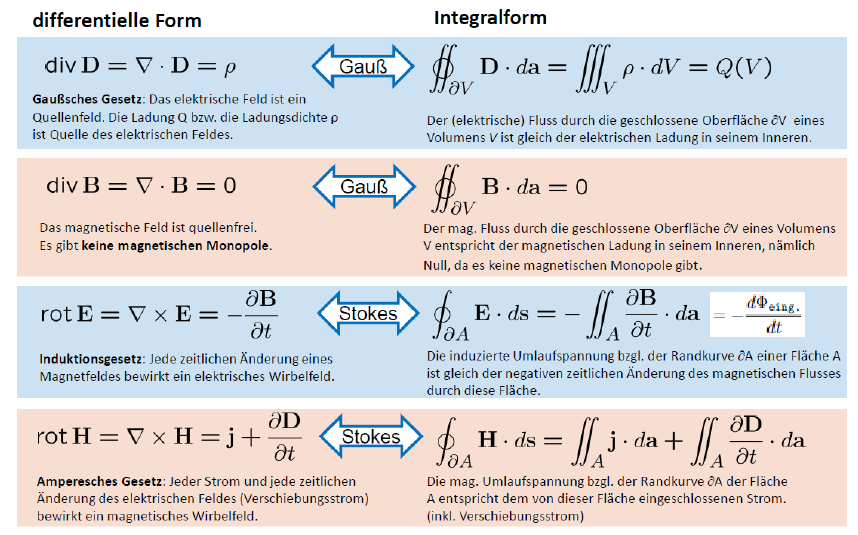
\includegraphics[width=\columnwidth]{Figures/Integralsatz.png}
% \subsection{stationäre Felder (Gleichstrom)}

% \begin{align*}
%     \nabla \cdot \vec{D}  & = \rho \qquad \vec{D} = \varepsilon \cdot \vec{E} \\
%     \nabla \times \vec{E} & = 0                                               \\
%     \nabla \times \vec{H} & = \vec{J} \qquad \vec{B} = \mu \cdot \vec{H}      \\
%     \nabla \cdot \vec{B}  & = 0                                               \\
% \end{align*}

% \subsection{statische Felder}
% Elektrostatik: $\vec{J} = 0$\\
% $\operatorname{rot} \vec{E} = 0$\\
% Magnetostatik: $\vec{J} = const$
